\begin{frame}{Leading thought}
    \begin{center}
        \alert{
            All computation is wrong, only some is useful.
        }
    \end{center}
    \vspace{4em}
    \begin{center}
        So far so obvious, but to what extend should one care?\\[1em]
    \visible<2>{
        \textcolor{grey5}{\smaller Or: Why should I devote a full semester to this topic?}
    }
    \end{center}
\end{frame}

\begin{frame}{Why care ? \quad Let's say your future job involves to \ldots}
    \begin{columns}[T]
        \smaller
    \begin{column}{0.3\textwidth}
    \begin{block}{Launch a rocket}
        \begin{center}
        \begin{tikzpicture}
            \node at (0, 0) {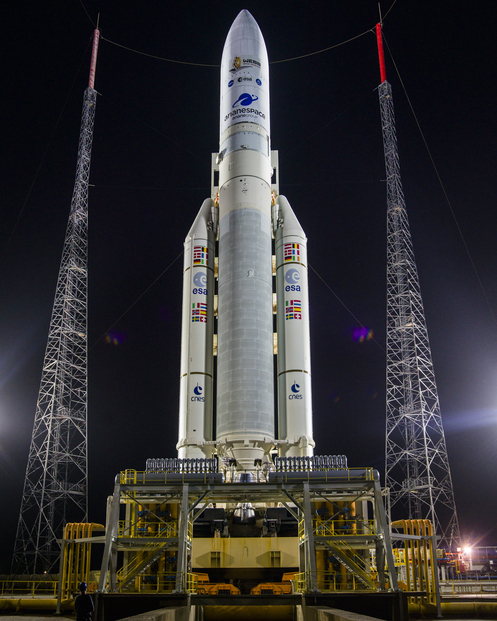
\includegraphics[width=0.8\textwidth]{img/disasters/Ariane_5.jpg}};
            \only<2->{\node [fill=white,rotate=40]  at (0, 0) {\alert{Self-destructed}};}
        \end{tikzpicture}
        \end{center}
        \visible<2->{
        \begin{itemize}
            \item June 1996
            \item Ariane 5 test
            \item 500 million dollar
            \visible<3->{
                \item \alert{floating point conversion error}
            }
        \end{itemize}
        }
    \end{block}
    \end{column}

    \begin{column}{0.3\textwidth}
    \begin{block}{Build an oil rig}
        \begin{center}
            \begin{tikzpicture}
                \node at (0, 0) {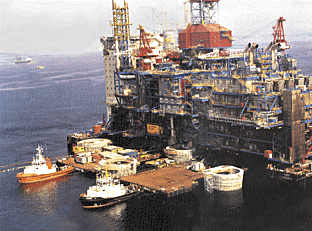
\includegraphics[width=\textwidth]{img/disasters/sleipner.png}};
                \only<2->{\node [fill=white,rotate=40]  at (0, 0) {\alert{Broken and sunken}};}
        \end{tikzpicture}
        \end{center}
        \visible<2->{
        \begin{itemize}
            \item August 1991
            \item Sleipner A offshore platform
            \item 1 billion dollar
            \visible<3->{
            \item \alert{Too crude discretisation}
            }
        \end{itemize}
        }
    \vspace{0.7em}
    \end{block}
    \end{column}

    \begin{column}{0.3\textwidth}
    \begin{block}{Intercept a missile}
        \begin{tikzpicture}
            \node at (0, 0) {
                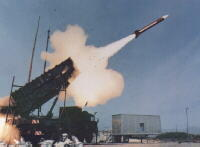
\includegraphics[width=\textwidth]{img/disasters/patriot.jpg}
            };
            \only<2->{\node [fill=white,rotate=40]  at (0, 0) {\alert{Missed Iranian missile}};}
        \end{tikzpicture}
        \visible<2->{
            \vspace{-1.0em}
        \begin{itemize}
            \item February 1991
            \item Patriot missile failure
            \item 28 soldiers killed, 100 injured
            \visible<3->{
            \item \alert{floating point conversion error}
            }
        \end{itemize}
        }
    \end{block}
    \end{column}
    \end{columns}

    \visible<3>{
    \vspace{1.0em}
    \begin{itemize}
            \smaller[2]
        \item See website of Douglas N. Arnold for more details:
            \url{https://www-users.cse.umn.edu/~arnold/disasters/disasters.html}
    \end{itemize}
    }
\end{frame}

\begin{frame}{Ok, so these are the extreme cases, right?}
    \begin{center}
        \larger
        \alert{Brainstorming:} Sources of error in scientific simulations
    \end{center}
    \vspace{3.0em}
    \visible<2>{
    \begin{itemize}
        \item Model
        \item Numerics \textcolor{grey5}{\smaller (discretisation / basis set, algorithm, arithmetic)}
        \item Implementation
        \item Hardware \textcolor{grey5}{\smaller (CPUs have bugs!)}
    \end{itemize}
    }
\end{frame}


%
% MatMat motivation
%

\begin{frame}{Motivation in the \matmat group}
    \begin{itemize}
        \item \alert{21st century challenges}:
            \begin{itemize}
                \vspace{-0.3em}
                \item Renewable energy, green chemistry, health care \ldots
            \end{itemize}
        \vspace{0.2em}
        \item Current solutions limited by properties of available materials
            \begin{itemize}
                \vspace{-0.3em}
                \item[$\Rightarrow$] Innovation driven by \alert{discovering new materials}
            \end{itemize}
        \vspace{0.2em}
        \item Crucial tool: \alert{Computational materials discovery}
            \begin{itemize}
                \vspace{-0.3em}
                \item Systematic simulations on \alert{$\simeq 10^4 - 10^6$ compounds}
                \vspace{-0.3em}
                \item Complemented by data-driven approaches
                \vspace{-0.3em}
                \item \alert{Noteworthy share} of world's supercomputing resources
            \end{itemize}
    \end{itemize}
    \vspace{0.2em}
    \definecolor{pgray}{rgb}{0.169,0.169,0.251}
    \begin{center}
        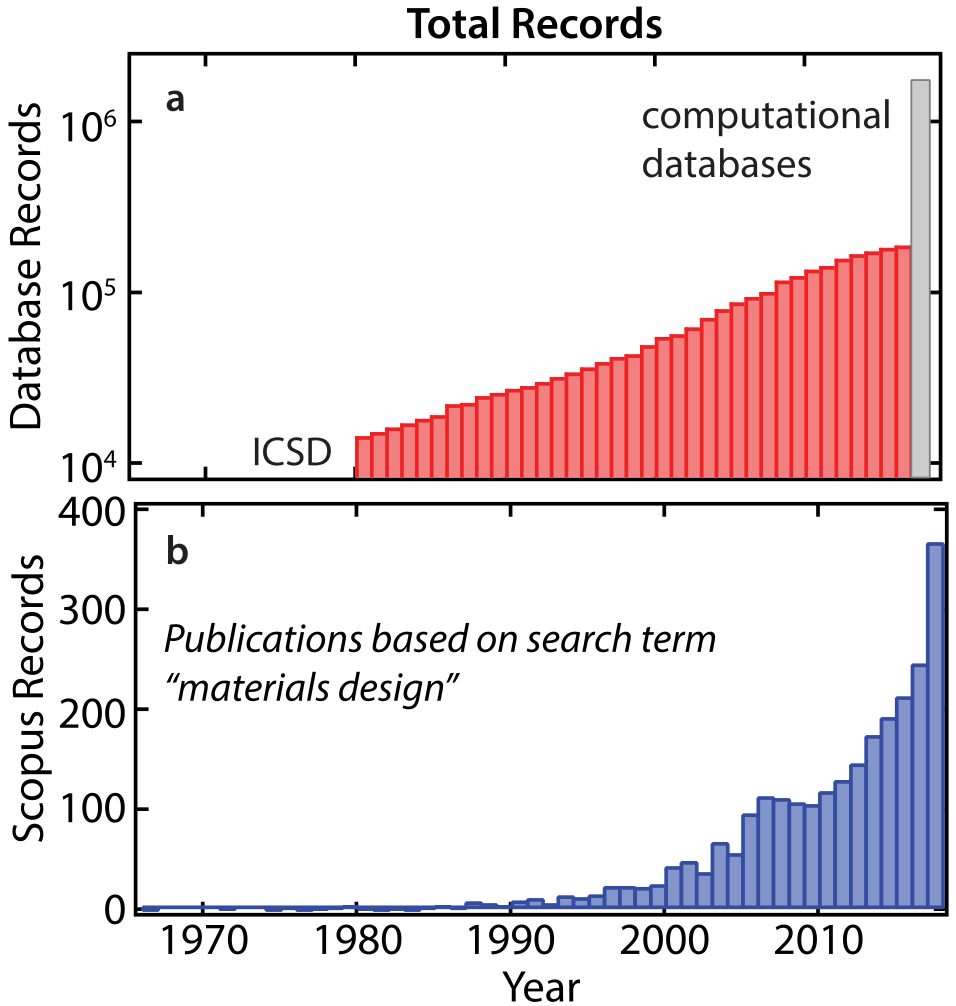
\includegraphics[height=3.3cm]{img/intro/roadmap-growth.png}
        \hspace{1.5em}
        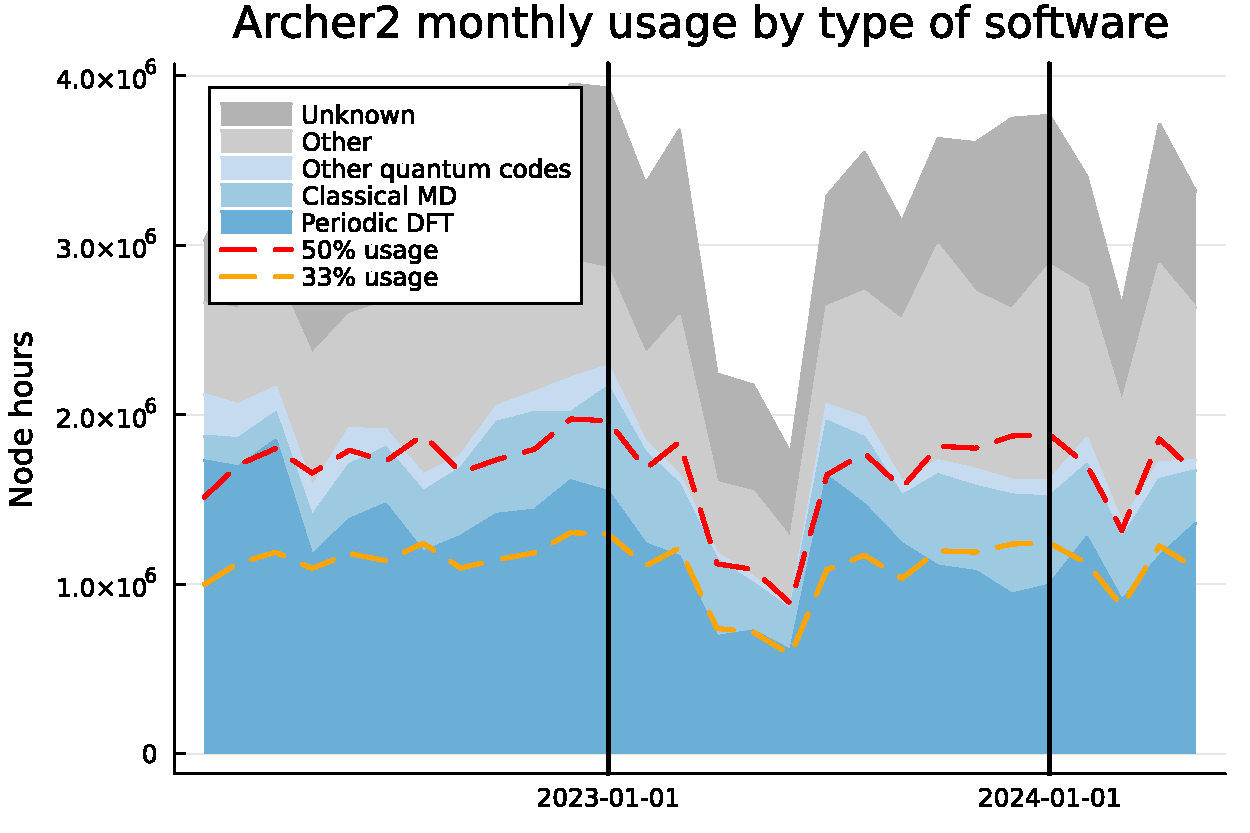
\includegraphics[height=3.3cm]{img/intro/archer_usage.pdf}
    \end{center}
   \vspace{-1.3em}
   \rule{4.5cm}{0.5pt}\\[-0.5em]
   {\tiny \href{http://dx.doi.org/10.1088/1361-6463/aad926}{%
       K. Alberi \textit{et. al.} J. Phys. D, \textbf{52}, 013001 (2019).}}
\end{frame}


\begin{frame}{Does everything need to be equally accurate ?}
    %\vspace{-0.5cm}
    \begin{center}
       \definecolor{oldorange}{HTML}{ee6322}
       \colorlet{myorange}{MfhGreen!65!MfhDarkGreen}
        \begin{tikzpicture}[inner sep=0cm]
            \node at (-5, 0.3) {
                \begin{lpic}[r(2.5cm)]{img/intro/funnel.png(.1)}
                    \lbl[l]{232,153;$\Big\}$\smaller[3] lowest-cost filter}
                    \lbl[l]{203, 95;\smaller[3]progressively...}
                    \lbl[l]{187, 60;\smaller[3]more...}
                    \lbl[l]{175, 25;\smaller[3]computational expense...}
                \end{lpic}
            };
            \node at (-4.86, -1.3) (new) {\smaller[2.5] \textcolor{myorange}{\textbf{\ New material candidates}}};
            \draw [->,myorange,thick] (new.west) ++ (1, 3.5) .. controls +(-1,-1) .. (new.west);
            \draw [->,myorange,thick] (new.west) ++ (-1, 3.5) .. controls +(1,-1) .. (new.west);
            \draw [->,myorange,thick] (new.west) ++ (-0.5, 3.5) .. controls +(0.5,-1) .. (new.west);
            \draw [->,myorange,thick] (new.west) ++ (0.5, 3.5) .. controls +(-0.5,-1) .. (new.west);
            \draw [->,myorange,thick] (new.west) ++ (-1.5, 3.5) .. controls +(1.5,-1) .. (new.west);
            \draw [->,myorange,thick] (new.west) ++ (1.5, 3.5) .. controls +(-1.5,-1) .. (new.west);
            \node at (-5.5, -1.9) {\smaller[3.5] Computational materials design funnel};
            \node at (-5.5, -2.17)
            {\smaller[3.5] \textcolor{grey5}{Involved data-driven multi-physics workflows}};


            \begin{scope}[xshift=-0.3cm]
            \node at (0, 0.3) {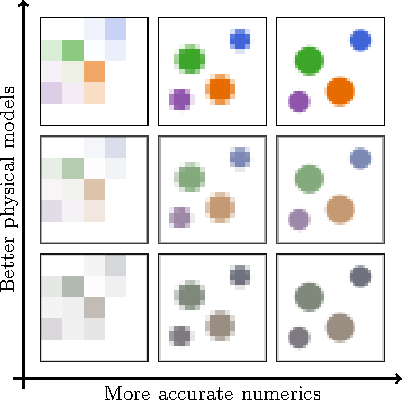
\includegraphics[width=3.7cm]{img/intro/error_flavours_9.pdf}};
            \node at (0, -1.9) {\smaller[3.5] Multitude of modelling choices};
            \node at (0, -2.2)
            {\smaller[3.5] \textcolor{grey5}{How should we spent our efforts best ?}};
            % \node at (0, -2.5)
            % {\smaller[3.5] \textcolor{grey5}{Can we make some computations less accurate ?}};
            \end{scope}
        \end{tikzpicture}
    \end{center}
    % \vspace{0.1em}
    \visible<2>{
        \begin{block}{\textcolor{black}{\textbf{Goal} in \matmat group:} \alert{Error-controled robust algorithms}}
        \begin{itemize}
        \smaller[0.5]
        \item Many parameters to choose \textcolor{grey5}{(algorithms, tolerances, models)}
        \item Need balance: Too expensive $\leftrightarrow$ Insufficient reliability
        \item[$\Rightarrow$] \alert{Trial and error process !}
        \vspace{0.8em}
        \item Transform \alert{empirical wisdom} to built-in \alert{convergence guarantees}
        \item Requires: Uncertainty quantification \& error estimation
        \item[$\Rightarrow$] Understand \alert{where and how} to spend efforts best
        \end{itemize}
        \vspace{-0.2em}
    \end{block}
    }
\end{frame}

\begin{frame}{\matmat Advances in error estimation for materials models}
    \begin{center}
        \begin{tikzpicture}[inner sep=0cm]
            \node (bands) at (0, 0) {
            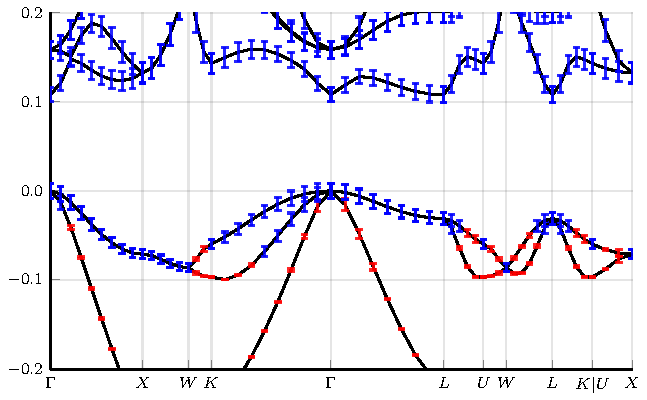
\includegraphics[width=4cm]{img/si_band_errors.pdf}
        };
        \node [below=0.1cm of bands] {\smaller[3.5] Band structure with \alert{guaranteed error bars}\footnotemark[1]};

        \node [right=5cm of bands.south, anchor=south,yshift=0.5cm] (uq) {
            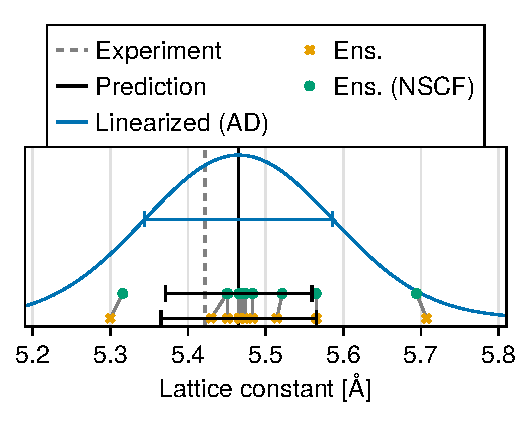
\includegraphics[width=4cm,trim=0 10 0 70,clip]{%
            img/Si_lattice_const_uncertainty_beef.pdf}
        };
        \node [below=0.1cm of uq] {\smaller[3.5] DFT lattice constant \alert{error distribution}\footnotemark[2]};

        \node [below=4.6cm of bands.south, anchor=south] (force) {
            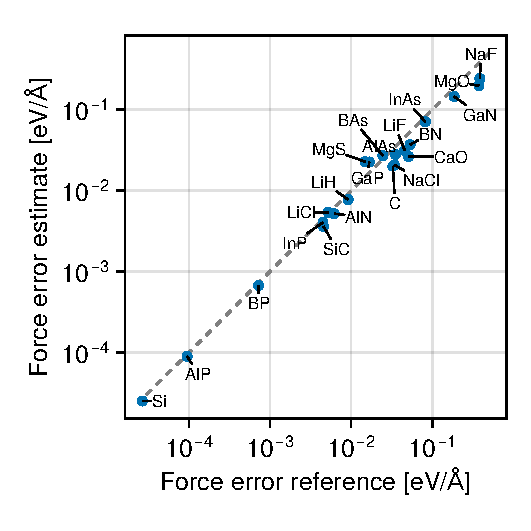
\includegraphics[width=4cm]{img/pw_error_estimation_force.pdf}
        };
        \node [below=-0.15cm of force] {\smaller[3.5] Plane-wave \alert{basis error estimates} at 20Ha\textsuperscript{2,3}};

        \node [right=5cm of force.south, anchor=south,yshift=0.25cm] (combin) {
            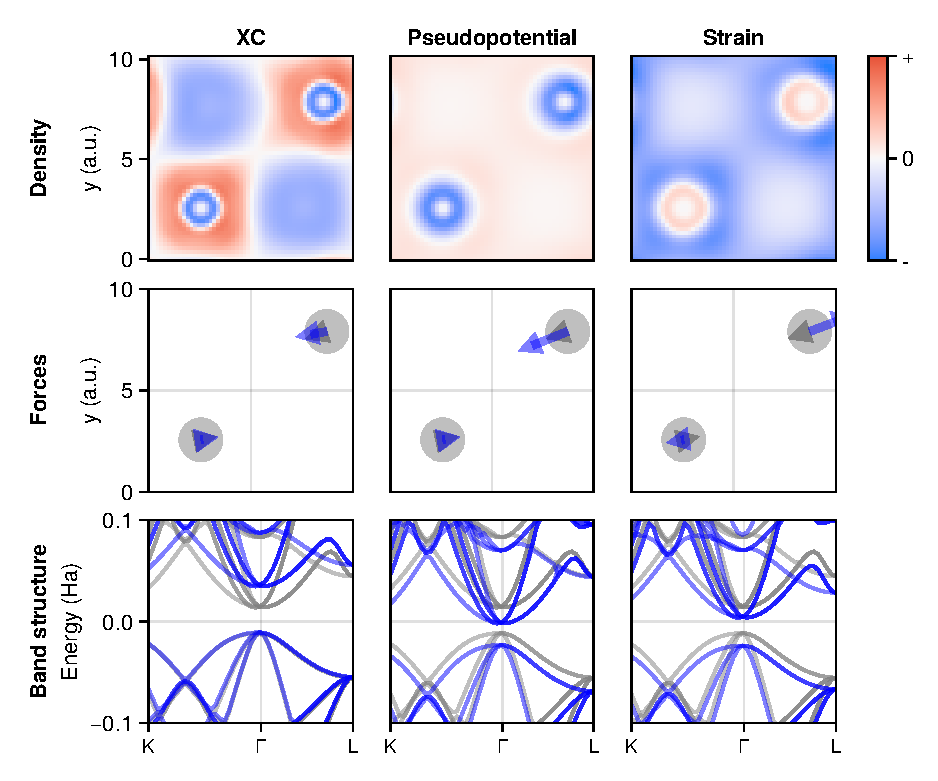
\includegraphics[width=4.5cm]{img/silicon_Ecut30_kgrid4_combined_density_forces_bands.pdf}
        };
        \node [below=0.1cm of combin] {\smaller[3.5] DFT quantity vs.~\alert{parameter sensitivities}\footnotemark[2]};
        \end{tikzpicture}
    \end{center}
    \visible<2>{%
    \begin{tikzpicture}[remember picture,overlay]
        \node [anchor=center,fill=grey9,rounded corners,inner sep=3mm] at (current page.center) {
            \begin{minipage}{\textwidth}
                Towards \textbf{inexact computation without harm}:
                \begin{itemize}
                    \vspace{0.1em}
                    \item Error remains controllable
                    \vspace{0.1em}
                    \item Challenge:
                        Turning \alert{mathematical analysis
                        into practical tool}
                        \begin{itemize}
                            \item Needs performance tuning, heuristics, best practices, \ldots
                        \end{itemize}
                    \vspace{0.6em}
                    \item \alert{Opportunities:} %High-level overview of current state
                        \begin{itemize}
                            \item Track simulation uncertainties
                            \item Learn missing physics
                            \item Leverage inexactness
                        \end{itemize}
                \end{itemize}
            \end{minipage}
        };
    \end{tikzpicture}
    }%
    \vspace{-1em}
    \footnotetext[1]{\papererror}
    \footnotetext[2]{\paperdftkad}
    \footnotetext[3]{\href{https://doi.org/10.1137/21M1456224}{%
         E. Cancès, G.~Dusson, G.~Kemlin \textit{et. al.} SIAM J. Sci. Comp., \textbf{44}, B1312 (2022).}}
\end{frame}

\begin{frame}{Questions ?}
    \begin{center}
        \huge{Questions ?}
    \end{center}
\end{frame}

\begin{frame}{Focus of the course: Eigenvalue problems}
    \begin{itemize}
        \item Eigenvalue problems are ubiquitous, e.g.
        \vspace{2em}
        \item \alert{Vibrations of structures}
            \begin{itemize}
                \item Tacoma narrows bridge collapse 1940
                \item London millennium bridge construction flaw
            \end{itemize}
        \vspace{1em}
        \item \alert{Quantum states} \textcolor{grey5}{\smaller (details follow)}
        \vspace{1em}
        \item Tight relation to \alert{linear problems \& PDEs}
            \begin{itemize}
                \item Convergence analysis (CG, iterative methods)
                \item Quantum mechanics
                \item Close relation to solving PDEs
                    \textcolor{grey5}{\smaller (details follow)}
            \end{itemize}
    \end{itemize}
\end{frame}
